Voor de navigatie was het voldoende om het nieuw project aan te maken. 
Hierbij zit de navigatie al geïmplemnteerd.

\paragraph{1. Gradle instellingen aanpassen}
Om de SplashScreen API te gebruiken, moeten we deze aan onze dependacies toevoegen. Dit doen we in
het \textbf{build.gradle(module)} bestand.
\begin{minted}{kotlin}
dependencies {
    // andere dependacies
    implementation("androidx.core:core-splashscreen:1.0.0")
}
\end{minted}

\paragraph{2. SplashScreen instellen}
Na het toevoegen van de dependancy kunnen we het laadscherm customizen op basis van onze wensen. 
Hiervoor maken we een nieuw \textbf{splash.xml} bestand in de \textbf{res/values} map. In dit 
bestand kunnen we dan het laadscherm customizen. Ook voegen we hier een icon toe dat zal worden
getoond tijdens het laden. Dit icoon moet in de \textbf{res/drawable} map worden geplaatst.
\begin{minted}{xml}
<?xml version="1.0" encoding="utf-8"?>
<resources>
    <style name="Theme.MyApp.MySplash" parent="Theme.SplashScreen">
        <item name="windowSplashScreenBackground">@color/black</item>
        <item name="windowSplashScreenAnimatedIcon">
            @drawable/bank_svgrepo_com</item>
        <item name="postSplashScreenTheme">@style/Theme.Basis</item>
    </style>
</resources>
\end{minted}

\paragraph{3. Applicatie maken}
Dankzij deze informatie kunnen we een applicatie opzetten dat een laadscherm toont dat zal verdwijnen 
van zodra de applicatie zijn eerste frame tekent. Daarna is er een navigatiebar te zien onderaan die ervoor zorgt dat 
we kunnen navigeren tussen de verschillende schermen.
\begin{figure}[H]
    \centering
    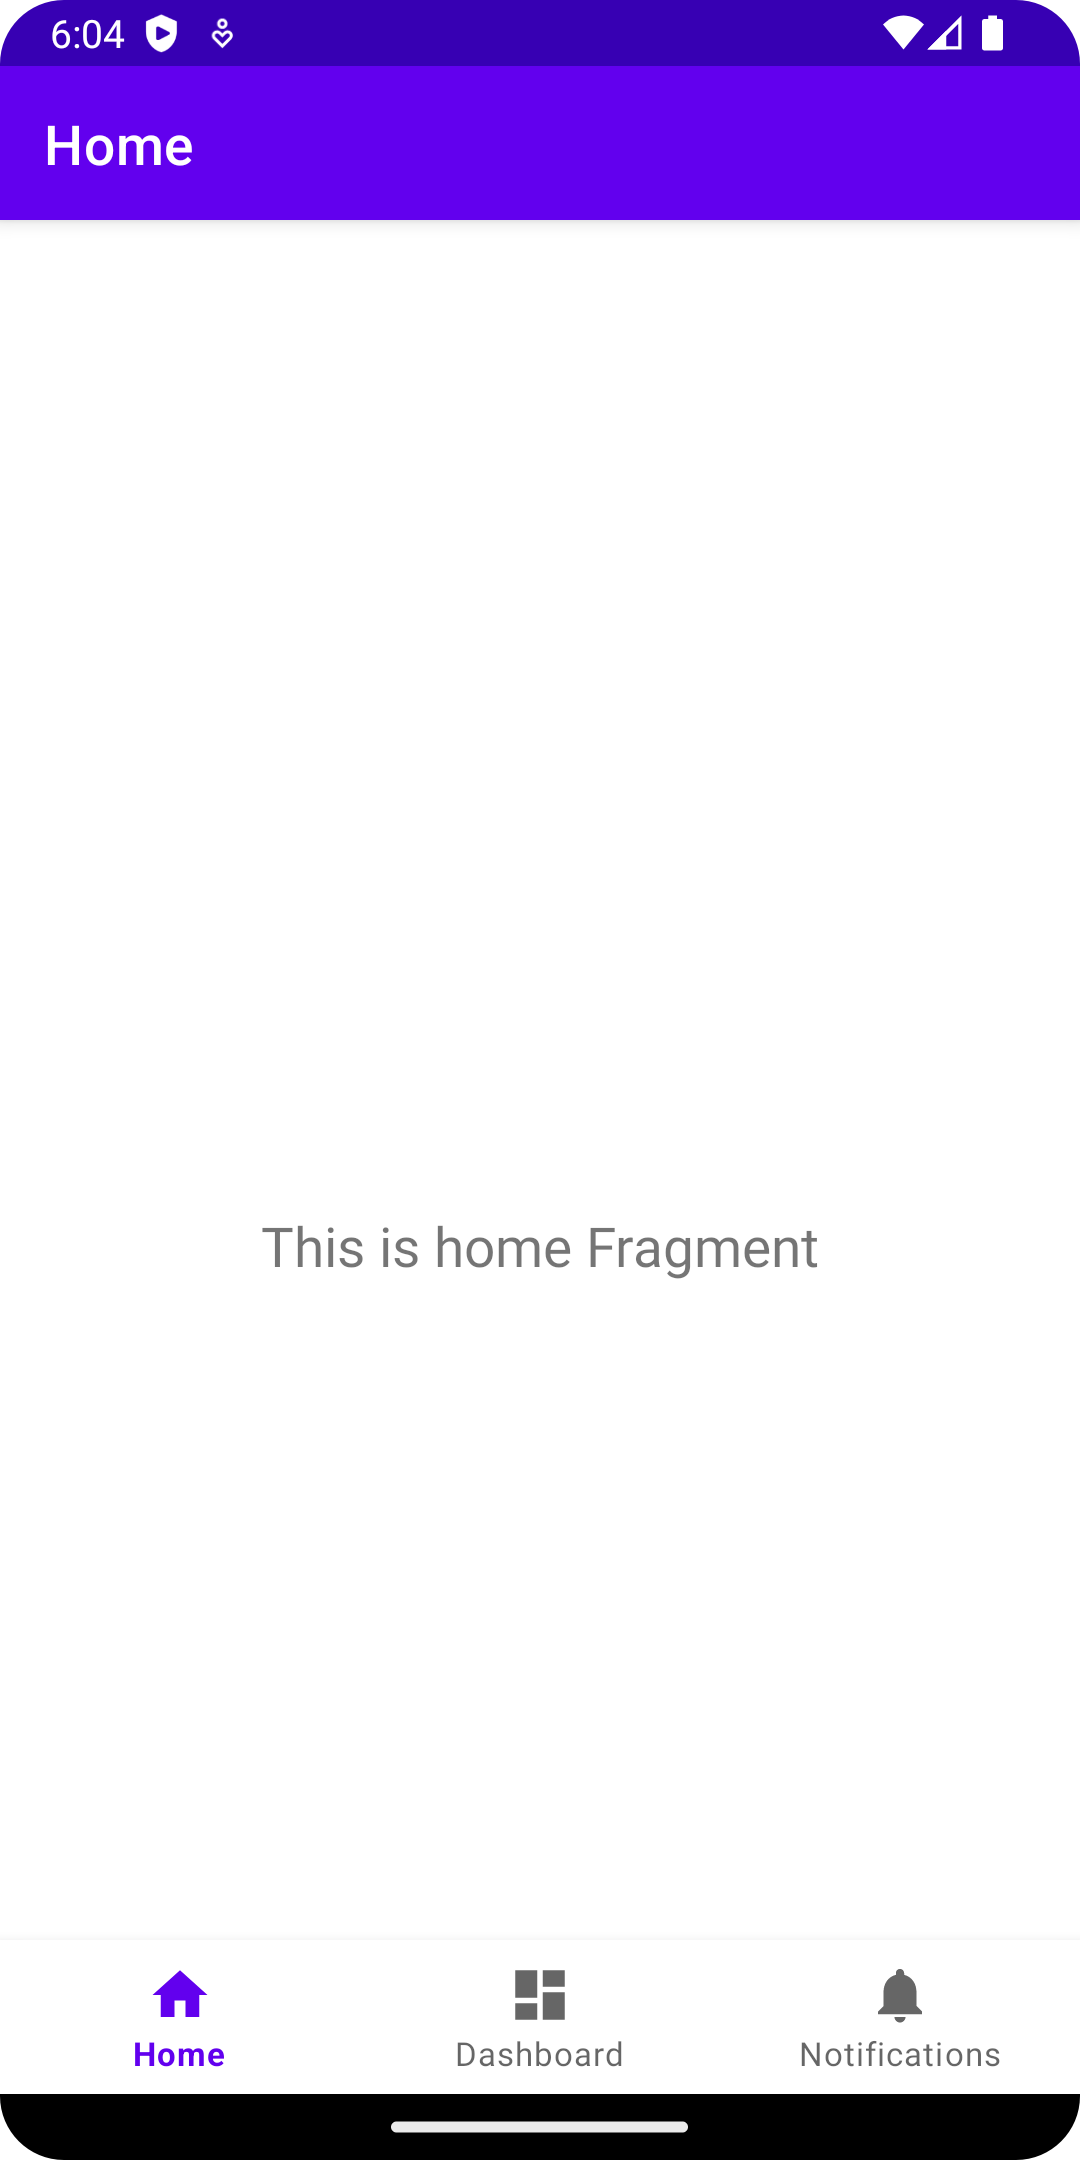
\includegraphics[height=0.4\textheight]{basis_layoutnative.png}
    \caption{Layout van applicatie voor de basisfunctionaliteiten bij Android.}
\end{figure}
